\documentclass[12pt, letterpaper]{article}
\usepackage{amsmath}  % Enhanced math package
\usepackage{amsfonts}  % Math fonts package
\usepackage{amssymb}  % Additional math symbols
\usepackage{geometry}  % Package for setting page dimensions
\usepackage{bm}
\usepackage{textcomp}
\usepackage{graphicx}
\usepackage{caption} % for \captionof

\geometry{top=1in, bottom=1in, left=1in, right=1in}

\title{\textbf{\Large TPK4171 - Advanced Industrial Robotics Exercise 1, 2024}}
\author{Joel Perurena}
\date{January 24, 2024}

\begin{document}
\maketitle
\section*{\large Problem 1}
The camera model is given by
\begin{equation}
    \bm{\tilde{s}=\frac{1}{z}r} \label{eq:normalized image coordinate}
\end{equation}

\begin{equation}
    \bm{\tilde{p}=K\tilde{s}} \label{eq:pixel coordinate}
\end{equation}

The camera parameter matrix is
\begin{equation}
    \bm{K}=\begin{bmatrix}
            k & 0 & u_0\\
            0 & k & v_0\\
            0 & 0 & 1
            \end{bmatrix} \label{eq:camera parameter matrix}
\end{equation}

The inverse of the camera parameter matrix is
\begin{equation}
    \bm{K^{-1}}=\begin{bmatrix}
            1/k & 0 & -u_0/k\\
            0 & 1/k & -v_0/k\\
            0 & 0 & 1
            \end{bmatrix} \label{eq:inverse camera parameter matrix}
\end{equation}

\begin{enumerate}
    \renewcommand{\labelenumi}{\alph{enumi})}
    \item The camera parameters given by the problem are 
    $k=1500$, $u_0=640$ and $v_0=512$, and the 3D points are given by
        \begin{equation*}
            \bm{r_1}=\begin{bmatrix}
                    0.1\\
                    0.2\\
                    0.5 
                    \end{bmatrix},
            \bm{r_2}=\begin{bmatrix}
                    1\\
                    2\\
                    5 
                    \end{bmatrix}
            \bm{r_3}=\begin{bmatrix}
                    0.1\\
                    0.2\\
                    1 
                    \end{bmatrix}
        \end{equation*}
        Find $\bm{\tilde{s}_1}$, $\bm{\tilde{s}_2}$ and $\bm{\tilde{s}_3}$ and $\bm{\tilde{p}_1}$, $\bm{\tilde{p}_2}$ and $\bm{\tilde{p}_3}$.
        
        From Equation \eqref{eq:normalized image coordinate} 
        we can compute $\bm{\tilde{s}_1}$, $\bm{\tilde{s}_2}$ and $\bm{\tilde{s}_3}$, 
        but first we need to know the value of $\bm{z}$. This value can be found just 
        taking the third value of the 3D points $\bm{r_1}$, $\bm{r_2}$ and $\bm{r_3}$.

        So knowing this, we can compute the values for $\bm{\tilde{s}_1}$, 
        $\bm{\tilde{s}_2}$ and $\bm{\tilde{s}_3}$ from Equation 
        \eqref{eq:normalized image coordinate}.
        \begin{equation*}
            {\tilde{s_1}=\frac{1}{z_1}r_1}=
            \frac{1}{0.5}\begin{bmatrix}
                        0.1\\
                        0.2\\
                        0.5 
                        \end{bmatrix}=
                        \begin{bmatrix}
                            0.2\\
                            0.4\\
                            1
                        \end{bmatrix}
        \end{equation*}

        \begin{equation*}
            {\tilde{s_2}=\frac{1}{z_2}r_2}=
            \frac{1}{5}\begin{bmatrix}
                        1\\
                        2\\
                        5 
                        \end{bmatrix}=
                        \begin{bmatrix}
                            0.2\\
                            0.4\\
                            1
                        \end{bmatrix}
        \end{equation*}

        \begin{equation*}
            {\tilde{s_3}=\frac{1}{z_3}r_3}=
            \frac{1}{1}\begin{bmatrix}
                        0.1\\
                        0.2\\
                        1 
                        \end{bmatrix}=
                        \begin{bmatrix}
                            0.1\\
                            0.2\\
                            1
                        \end{bmatrix}
        \end{equation*}

        Now that we have computed the values for the normalized image coordinates 
        we can compute the values for the pixel coordinates because we already have
        the values of $\bm{\tilde{s}_1}$, $\bm{\tilde{s}_2}$ and $\bm{\tilde{s}_3}$.
        Using \eqref{eq:pixel coordinate} and the values of the camera 
        parameters stated at the beggining we get
        \begin{equation*}
            {\tilde{p_1}=K\tilde{s_1}}=
            \begin{bmatrix}
                1500 & 0 & 640\\
                0 & 1500 & 512\\
                0 & 0 & 1
            \end{bmatrix}
            \begin{bmatrix}
                0.2\\
                0.4\\
                1
            \end{bmatrix}=
            \begin{bmatrix}
                940\\
                1112\\
                1
            \end{bmatrix}
        \end{equation*}

        \begin{equation*}
            {\tilde{p_2}=K\tilde{s_2}}=
            \begin{bmatrix}
                1500 & 0 & 640\\
                0 & 1500 & 512\\
                0 & 0 & 1
            \end{bmatrix}
            \begin{bmatrix}
                0.2\\
                0.4\\
                1
            \end{bmatrix}=
            \begin{bmatrix}
                940\\
                1112\\
                1
            \end{bmatrix}
        \end{equation*}

        \begin{equation*}
            {\tilde{p_3}=K\tilde{s_3}}=
            \begin{bmatrix}
                1500 & 0 & 640\\
                0 & 1500 & 512\\
                0 & 0 & 1
            \end{bmatrix}
            \begin{bmatrix}
                0.1\\
                0.2\\
                1
            \end{bmatrix}=
            \begin{bmatrix}
                790\\
                812\\
                1
            \end{bmatrix}
        \end{equation*}

    \item With pixel points
        \begin{equation*}
            \bm{\tilde{p}_a}=\begin{bmatrix}
                0\\
                0\\
                1
            \end{bmatrix},
            \bm{\tilde{p}_b}=\begin{bmatrix}
                740\\
                612\\
                1
            \end{bmatrix},
            \bm{\tilde{p}_c}=\begin{bmatrix}
                1280\\
                1024\\
                1
            \end{bmatrix}
        \end{equation*}

        It is posible to compute the normalized image coordinates
        $\bm{\tilde{s}_a}$, $\bm{\tilde{s}_b}$ and $\bm{\tilde{s}_c}$ by using
        Equation \eqref{eq:pixel coordinate} and solving for $\bm{\tilde{s}}$
        \begin{equation*}
            \bm{\tilde{s}=K^{-1}\tilde{p}}
        \end{equation*}
        
        Using Equation \eqref{eq:inverse camera parameter matrix} we can compute 
        for the normalized image coordinates
        \begin{equation*}
            \tilde{s}_a=K^{-1}\tilde{p}_a=\begin{bmatrix}
                1/1500 & 0 & -640/1500\\
                0 & 1/1500 & -512/1500\\
                0 & 0 & 1
            \end{bmatrix}
            \begin{bmatrix}
                0\\
                0\\
                1
            \end{bmatrix}=\begin{bmatrix}
                -0.427\\
                -0.341\\
                1
            \end{bmatrix}
        \end{equation*}

        \begin{equation*}
            \tilde{s}_b=K^{-1}\tilde{p}_b=\begin{bmatrix}
                1/1500 & 0 & -640/1500\\
                0 & 1/1500 & -512/1500\\
                0 & 0 & 1
            \end{bmatrix}
            \begin{bmatrix}
                740\\
                612\\
                1
            \end{bmatrix}=\begin{bmatrix}
                0.067\\
                0.067\\
                1
            \end{bmatrix}
        \end{equation*}

        \begin{equation*}
            \tilde{s}_c=K^{-1}\tilde{p}_c=\begin{bmatrix}
                1/1500 & 0 & -640/1500\\
                0 & 1/1500 & -512/1500\\
                0 & 0 & 1
            \end{bmatrix}
            \begin{bmatrix}
                1280\\
                1024\\
                1
            \end{bmatrix}=\begin{bmatrix}
                0.427\\
                0.341\\
                1
            \end{bmatrix}
        \end{equation*}

    \item The displacement of the oject frame $o$ with respect to the camera frame 
            $c$ is given by
            \begin{equation}
                \bm{T^{c}_o}=\begin{bmatrix}
                    \bm{R^{c}_o} & \bm{t^{c}_co}\\
                    \bm{0^{T}} & 1
                \end{bmatrix}
            \end{equation}
            Where
            \begin{equation*}
                \bm{t^{c}_{co}}=[0,0,4]^T
            \end{equation*}
            and
            \begin{equation*}
                \bm{R^{c}_o}=\bm{R_x}(\pi/2)=
                \begin{bmatrix}
                    1 & 0 & 0 \\
                    0 & \cos(\theta) & -\sin(\theta) \\
                    0 & \sin(\theta) & \cos(\theta)
                \end{bmatrix}=
                \begin{bmatrix}
                    1 & 0 & 0 \\
                    0 & \cos(\pi/2) & -\sin(\pi/2) \\
                    0 & \sin(\pi/2) & \cos(\pi/2)
                \end{bmatrix}=
                \begin{bmatrix}
                    1 & 0 & 0 \\
                    0 & 0 & -1 \\
                    0 & 1 & 0
                \end{bmatrix}
            \end{equation*}
            A point $P$ is given by its position $\bm{r^{o}_{op}}=[1,1,0]^T$
            in the object frame. With this information find the matrix $\bm{C}$
            that satisfies the following expression.
            \begin{equation}
                z\bm{\tilde{s}=C\tilde{r}_{op}^{o}} \label{eq:C}
            \end{equation}
            %Find C to safisfy z*s=C*ro_p in this case C=[Rc_o tc_o] E R3x4
            This $\bm{C}$ matrix can be found by looking at Equation (25) from
            the Vision.pdf provided by Professor Olav Egeland
            \begin{equation}
                \bm{\tilde{s}=}\frac{1}{z}\bm{\Pi T_o^c\tilde{r}^o_{op}}
            \end{equation}
            This equation can be written in another way by multiplying all
            the equation by $\bm{z}$. This will result in the following equation
            \begin{equation}
                z\bm{\tilde{s}=\Pi T_o^c\tilde{r}^o_{op}}\label{eq:Pi}
            \end{equation}
            So now we can compare equations \eqref{eq:C} and \eqref{eq:Pi} and 
            observe that
            \begin{equation*}
                \bm{C}=\bm{\Pi T_o^c}
            \end{equation*}
            And from the Vision.pdf notes provided by Professor Olav Egeland we
            can know that
            \begin{equation*}
                \bm{\Pi T_o^c}=\begin{bmatrix}
                    \bm{R_o^c} & \bm{t^c_{co}}
                \end{bmatrix} \in \mathbb{R}^{3\times4}
            \end{equation*}
            Hence
            \begin{equation*}
                \bm{C}=\begin{bmatrix}
                    \bm{R_o^c} & \bm{t^c_{co}}
                \end{bmatrix} \in \mathbb{R}^{3\times4}
            \end{equation*}
            The values of $\bm{R_o^c}$ and $\bm{t^c_{co}}$ are given so $C$ can be
            computed
            \begin{equation*}
                \bm{C}=                
                \begin{bmatrix}
                    1 & 0 & 0 & 0\\
                    0 & 0 & -1 & 0\\
                    0 & 1 & 0 & 4
                \end{bmatrix}
            \end{equation*}
            Find the normalized image coordinates $\bm{\tilde{s}}$ and the pixel 
            coordinate $\bm{\tilde{p}}$ of point $P$.
            To compute this $z$ needs to be obtained first. This value is found
            by taking the third value of the vector $\bm{\tilde{r}^c_{cp}}$ which
            is defined by
            \begin{equation*}
                \bm{\tilde{r}^c_{cp}=T_o^c\tilde{r}^{o}_{op}}
            \end{equation*}
            Where 
            \begin{equation*}
                \bm{\tilde{r}^{o}_{op}}=
                \begin{bmatrix}
                    \bm{r^o_{op}}\\
                    1
                \end{bmatrix}=
                \begin{bmatrix}
                    1\\
                    1\\
                    0\\
                    1
                \end{bmatrix}
            \end{equation*}
            Hence
            \begin{equation*}
                \bm{\tilde{r}^c_{cp}=T_o^c\tilde{r}^{o}_{op}}=
                \begin{bmatrix}
                    1 & 0 & 0 & 0\\
                    0 & 0 & -1 & 0\\
                    0 & 1 & 0 & 4\\
                    0 & 0 & 0 & 1
                \end{bmatrix}
                \begin{bmatrix}
                    1\\
                    1\\
                    0\\
                    1
                \end{bmatrix}=
                \begin{bmatrix}
                    1\\
                    0\\
                    5\\
                    1
                \end{bmatrix}
            \end{equation*}
            From this result $\bm{\tilde{r}^c_{cp}}$ is obtained and $\bm{\tilde{s}}$ can be
            computed were $z=\bm{\tilde{r}^c_{cp}}(3)=5$
            \begin{equation*}
                \bm{\tilde{s}}=\frac{1}{z}\bm{{r}^c_{cp}}=
                \frac{1}{5}                
                \begin{bmatrix}
                    1\\
                    0\\
                    5
                \end{bmatrix}=
                \begin{bmatrix}
                    0.2\\
                    0\\
                    1
                \end{bmatrix}
            \end{equation*}
            And $\bm{\tilde{p}}$ can be computed with
            \begin{equation*}
                \bm{\tilde{p}}=\bm{K\tilde{s}}=
                \begin{bmatrix}
                    1500 & 0 & 640\\
                    0 & 1500 & 512\\
                    0 & 0 & 1
                \end{bmatrix}
                \begin{bmatrix}
                    0.2\\
                    0\\
                    1
                \end{bmatrix}=
                \begin{bmatrix}
                    940\\
                    512\\
                    1
                \end{bmatrix}
            \end{equation*}
\end{enumerate}
\section*{\large Problem 2}
A camera is used to find points in a horizontal plane. The displacement from
the camera frame to the object frame is given by
\begin{equation*}
    \bm{T^{c}_o}=\begin{bmatrix}
        \bm{R_x}(120^\circ) & \bm{t}\\
        \bm{0^{T}} & 1
    \end{bmatrix}
\end{equation*}
\begin{equation*}
    \bm{R_x}(120^\circ)=
    \begin{bmatrix}
        1 & 0 & 0 \\
        0 & \cos(120^\circ) & -\sin(120^\circ) \\
        0 & \sin(120^\circ) & \cos(120^\circ)
    \end{bmatrix}=
    \begin{bmatrix}
        1 & 0 & 0 \\
        0 & -\frac{1}{2} & -\frac{\sqrt[]{3}}{2} \\
        0 & \frac{\sqrt[]{3}}{2} & -\frac{1}{2}
    \end{bmatrix}
\end{equation*}
Where $\bm{t}=[0,0,2]^T$ and 4 points are given in the object frame as the corners of a 
quadratic rectangle with coordinates 
\begin{equation*}
    \bm{r_{o1}^c}=
    \begin{bmatrix}
        0\\
        0\\
        0
    \end{bmatrix},
    \bm{r_{o2}^c}=
    \begin{bmatrix}
        1\\
        0\\
        0
    \end{bmatrix},
    \bm{r_{o3}^c}=
    \begin{bmatrix}
        1\\
        1\\
        0
    \end{bmatrix},
    \bm{r_{o4}^c}=
    \begin{bmatrix}
        0\\
        1\\
        0
    \end{bmatrix}
\end{equation*}
\begin{enumerate}
    \renewcommand{\labelenumi}{\alph{enumi})}
    \item Find the coordinates $\bm{r_{c1}^c}$, $\bm{r_{c2}^c}$, $\bm{r_{c3}^c}$, 
        $\bm{r_{c4}^c}$ of the points of the camera frame.

        \begin{equation*}
            \bm{\tilde{r}^c_{c1}=T_o^c\tilde{r}^{o}_{o1}}=
            \begin{bmatrix}
                1 & 0 & 0 & 0\\
                0 & -\frac{1}{2} & -\frac{\sqrt[]{3}}{2} & 0\\
                0 & \frac{\sqrt[]{3}}{2} & -\frac{1}{2} & 2\\
                0 & 0 & 0 & 1
            \end{bmatrix}
                \begin{bmatrix}
                    0\\
                    0\\
                    0\\
                    1
                \end{bmatrix}=
                \begin{bmatrix}
                    0\\
                    0\\
                    2\\
                    1
                \end{bmatrix}
        \end{equation*}
        \begin{equation*}
            \bm{\tilde{r}^c_{c2}=T_o^c\tilde{r}^{o}_{o2}}=
            \begin{bmatrix}
                1 & 0 & 0 & 0\\
                0 & -\frac{1}{2} & -\frac{\sqrt[]{3}}{2} & 0\\
                0 & \frac{\sqrt[]{3}}{2} & -\frac{1}{2} & 2\\
                0 & 0 & 0 & 1
            \end{bmatrix}
                \begin{bmatrix}
                    1\\
                    0\\
                    0\\
                    1
                \end{bmatrix}=
                \begin{bmatrix}
                    1\\
                    0\\
                    2\\
                    1
                \end{bmatrix}
        \end{equation*}
        \begin{equation*}
            \bm{\tilde{r}^c_{c3}=T_o^c\tilde{r}^{o}_{o3}}=
            \begin{bmatrix}
                1 & 0 & 0 & 0\\
                0 & -\frac{1}{2} & -\frac{\sqrt[]{3}}{2} & 0\\
                0 & \frac{\sqrt[]{3}}{2} & -\frac{1}{2} & 2\\
                0 & 0 & 0 & 1
            \end{bmatrix}
                \begin{bmatrix}
                    1\\
                    1\\
                    0\\
                    1
                \end{bmatrix}=
                \begin{bmatrix}
                    1\\
                    -0.5\\
                    2.866\\
                    1
                \end{bmatrix}
        \end{equation*}
        \begin{equation*}
            \bm{\tilde{r}^c_{c4}=T_o^c\tilde{r}^{o}_{o4}}=
            \begin{bmatrix}
                1 & 0 & 0 & 0\\
                0 & -\frac{1}{2} & -\frac{\sqrt[]{3}}{2} & 0\\
                0 & \frac{\sqrt[]{3}}{2} & -\frac{1}{2} & 2\\
                0 & 0 & 0 & 1
            \end{bmatrix}
                \begin{bmatrix}
                    0\\
                    1\\
                    0\\
                    1
                \end{bmatrix}=
                \begin{bmatrix}
                    0\\
                    -0.5\\
                    2.866\\
                    1
                \end{bmatrix}
        \end{equation*}
    \item Find the normalized image coordinates of the points
        \begin{equation*}
            \bm{\tilde{s}_1}=\frac{1}{z}\bm{{r}^c_{c1}}=
            \frac{1}{2}
            \begin{bmatrix}
                0\\
                0\\
                2
            \end{bmatrix}=
            \begin{bmatrix}
                0\\
                0\\
                1
            \end{bmatrix}
        \end{equation*}
        \begin{equation*}
            \bm{\tilde{s}_2}=\frac{1}{z}\bm{{r}^c_{c2}}=
            \frac{1}{2}
            \begin{bmatrix}
                1\\
                0\\
                2
            \end{bmatrix}=
            \begin{bmatrix}
                0.5\\
                0\\
                1
            \end{bmatrix}
        \end{equation*}
        \begin{equation*}
            \bm{\tilde{s}_3}=\frac{1}{z}\bm{{r}^c_{c3}}=
            \frac{1}{2.866}
            \begin{bmatrix}
                1\\
                -0.5\\
                2.866
            \end{bmatrix}=
            \begin{bmatrix}
                0.349\\
                -0.174\\
                1
            \end{bmatrix}
        \end{equation*}
        \begin{equation*}
            \bm{\tilde{s}_4}=\frac{1}{z}\bm{{r}^c_{c4}}=
            \frac{1}{2.866}
            \begin{bmatrix}
                0\\
                -0.5\\
                2.866
            \end{bmatrix}=
            \begin{bmatrix}
                0\\
                -0.174\\
                1
            \end{bmatrix}
        \end{equation*}
    \item The rectangle is not quadratic in normalized image coordinates because there
        is an element of distortion due to the angle in which the picture is been taken.
        In the coordinates we can see that on the third value of the vectors $\bm{r_{c1}^c}$, $\bm{r_{c2}^c}$, $\bm{r_{c3}^c}$, 
        $\bm{r_{c4}^c}$ that would be the value related to the depth, the points 3 and 4 are
        deeper than the points 1 and 2, hence this will mean that in a plane, points
        1 and 2 will be farther away from each other compared to points 3 and 4, due to the fact 
        the factor of depth in the picture. If the camera would have been directly on top of the points, meaning that
        the depth would be the same for all 4 points, then the normalized coordinates will draw a perfect square.
\end{enumerate}
\newpage
\section*{\large Problem 3}
Use the Hough transform $\rho=x\cos\theta+y\sin\theta$ to find the lines
which corresponds to the data-set in Table 1. Sketch the curves, and find the line
with the highest number of points.
\begin{table}[ht]
    \centering
    \begin{tabular}{|c|c c c c c|}
        \hline
        Point & 1 & 2 & 3 & 4 & 5\\
        \hline
        $x$ & 0 & 1 & 2 & 3 & 0\\
        $y$ & 0 & 0 & 0 & 0 & 1\\
        \hline
    \end{tabular}
    \caption{Data-set for Hough transform} 
\end{table}
\begin{figure}[ht]
    \centering
    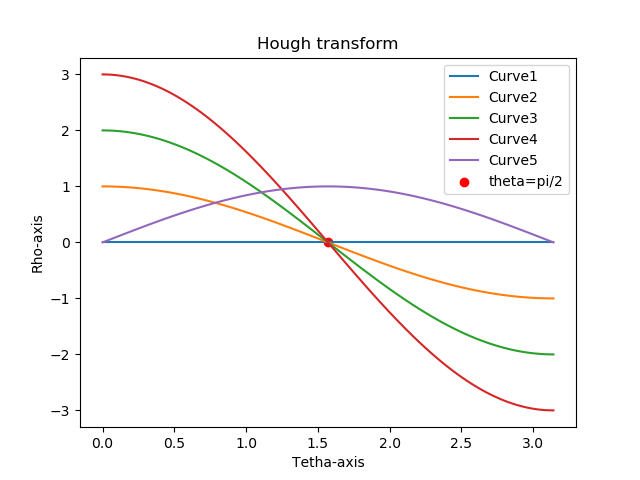
\includegraphics[width=0.8\linewidth]{Figure_1.png} % Replace "filename" with the actual name of your image file
    \caption{Plot of the sketched curves for each set of points.}
  \end{figure}
  From this plot it can be seen that the point in which most curves intersect
  is $\bm{P=(\rho,\theta)}=(0,\pi/2)$, this means that the line will be a line 
  through the origin orthogonal to $\pi/2$. Meaning it is an horizontal line $y=0$.
  \newpage
  \begin{figure}[ht]
    \centering
    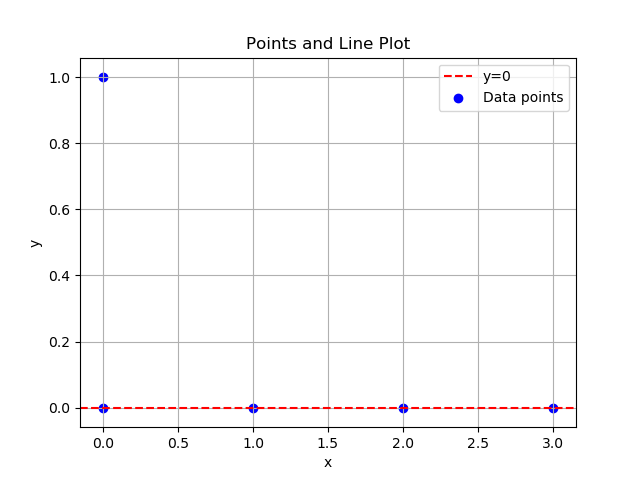
\includegraphics[width=0.8\linewidth]{Figure_2.png} % Replace "filename" with the actual name of your image file
    \caption{Plot of the sketched resulting line.}
  \end{figure}
\end{document}